%********** Chapter 3 **********
\chapter{Calculator\index{Calculator}}\index{projects!Calculator}

\section{Introduction}

This chapter introduces the second project, a calculator program.  The calculator's user can enter values and chose from a (initially very short) menu of available operations.  The program is designed to make it relatively easy to add additional operations.  The project introduces functions, which are basic mechanism for structuring code, and menu-driven programs, a very useful model for user interaction that is used in a wide range of  applications.

This project reviews the topics covered in Chapter 2 and introduces a number of new,  fundamental elements of programming, most notably:
\begin{tight_itemize}
  \item Functions\index{functions}
  \item Real numbers
\item Type Conversion and Casts
  \item Scope\index{scope}
  \item Switch statement\index{switch@{\cf{switch}}}
\end{tight_itemize}
Functions are separate blocks of code that have a particular role.  They can be used repeatedly and make it easier to design and write a program by breaking it into subtasks.  A new type, \codefont{double}, is introduced to hold real numbers.  Casts are used to convert numbers between different types.  Scope determines which variables can be used in which parts of a program.  A switch statement is a slightly more complex conditional that has multiple options instead of an if-else's two options.  

\section{The Program} 

Listings~\ref{listing:calc} and~\ref{listing:calcFunctions} present the code for a limited calculator.  Notice that the program is fairly short and is divided into several distinct sections.  Enter the code from \emph{both} Listings~\ref{listing:calc} and~\ref{listing:calcFunctions} as one long program.  (Again, do \emph{not} enter the line numbers; they are just for reference.)  As the program is entered, try to figure out what the statements do.  Many of them should be familiar from the previous programs; others will be new.  

Once the entire program has been entered, compile it.  As always, there may be some copying errors that need to be fixed.  Once the program compiles,  run it and see what it does.  Be sure to test all of the menu options and a variety of different numbers.  Are there any cases where the program produces an unexpected output?  What happens if a nonexistent menu option is tried?

\begin{minipage}{\textwidth}
\renewcommand*\thelstnumber{{\the\value{lstnumber}}}
\begin{lstlisting}[language=C++,numbers = left,xleftmargin=4.0ex, basicstyle=\small, emph={operand1,operand2,answer,choice,valid_choice},emphstyle = \color{\mycolor},
showstringspaces=false,
caption = {The code for the \codefont{main()} function and the prototypes for the other functions in the calculator program.},label = {listing:calc}]
/* A simple calculator program,
controlled by a menu and 
divided into separate functions */
#include<iostream>
using namespace std;
//---------- Function Prototypes -----------
void print_menu();
double get_value();
double divide(double,double);
//--------------  Main -------------------
int main()
{
     double operand1, operand2, answer;
     int choice, valid_choice;
     do{
           print_menu();
           cin >> choice;
           valid_choice = 1;           // assume choice is valid
           switch(choice){
           case 0:                    // program will exit
                  break;
           case 1:                    // addition
                  operand1 = get_value();
                  operand2 = get_value();
                  answer = operand1 + operand2;
                   break;
            case 2:                    // division
                   operand1 = get_value();
                   operand2 = get_value();
                   answer = divide(operand1,operand2);
                   break;
            default:
                   valid_choice = 0;   // choice is invalid
                   cout << "Invalid Choice." << endl;
            }
            if(valid_choice){   // if choice is valid, print the answer
                   cout << endl << "Answer = " << answer << endl;
            }
      }while(choice != 0);    // if not 0, loop back to start
      return 0;
}
\end{lstlisting}
\end{minipage}


As with NIM (and all of the other projects in this book) the program has some shortcomings that will need to be fixed.  Most notably, it doesn't have  many options for the user to choose from.  However, the program is written to make it easy to include additional options.  Being able to add functionality to a program is critical because it is very rare that a programmer knows in advance everything a program will eventually do.\footnote{You have probably noticed that commercial programs are often updated, patched, or replaced with new versions or expansions.  These are feasible only if the original program was written to be easily modifiable.}  Ideas for new functions and capabilities often occur either during programming or after the program's initial release.  Thus, when writing a program, it's important to make sure that it will be easy to expand and modify.

\begin{minipage}{\textwidth}
\renewcommand*\thelstnumber{\the\value{lstnumber}b}
\begin{lstlisting}[language=C++,numbers = left, xleftmargin=4.0ex, basicstyle=\small,emph={dividend, divisor,temp_value},emphstyle = \color{\mycolor},
showstringspaces=false,
caption = {The code for the functions that are used in the calculator program.  The lines are numbered followed by a \emph{`b'} for easy reference in the text.},
label={listing:calcFunctions}]
//--------------  Functions -------------------
double divide(double dividend, double divisor){
      if(divisor == 0)
            return 0;  // avoids divide by zero errors
      else
            return (dividend/divisor);
}
//----------------- get_value function ----------------
double get_value(){
      double temp_value;
      cout << "Enter a value: ";
      cin >> temp_value;
      return temp_value;
}
//-------------------- print_menu function -------------
void print_menu(){
     cout << endl;
     cout << "Add (1)" << endl;
     cout << "Divide (2)" << endl;
     cout << "Exit (0)" << endl;
     cout << "Enter your choice: ";
}
\end{lstlisting}
\end{minipage}


\subsection{Functions}\index{functions}
%\mysubsubsection{Lines 7-9, 1b-22b: Function Prototypes and Function Definitions}

Functions are a critical part of C++ programs.  A \emph{function} is a separate block of code that can be \emph{called} by other parts of the program when it is needed.  A function is a bit like a particular part in a larger machine that is used for a specific task.  The \codefont{rand()} function from Chapter~\ref{ch:NIM} is a good example -- when a random number is needed, the program calls the \codefont{rand()} function and it \emph{returns} a random number.  The \codefont{rand()} function contains some code, but the programmer generally doesn't have worry about how it works, so long as it returns a random number as expected.

When the computer reaches a function name, it immediately ``jumps'' to that function and begins executing the code within the function.  Then, when the computer either reaches a \emph{return} command within the function or the last closing brace \} of the function, it ``jumps'' back to where the function was called from.  For example, in the Calculator program, when the program reaches the command \codefont{get\_value()} on line 23, it jumps to line 9b, and then when it reaches line 14b, it jumps back to finish executing line 23.

Functions can take arguments\index{arguments}\index{functions!arguments}.  An \emph{argument} is one or more values that are handed to (or input to) the function for it to use.  Inside the function, the argument values are stored in variables called \emph{parameters}.\index{parameters}\index{functions!parameters}
Functions can easily be identified in code by the parentheses that follow them.  For example, \cf{move()} is a function because it has parentheses, whereas \cf{move} is a variable.  Thus, \cf{move()} is going to cause the program to jump to another piece of code (i.e., to to the \cf{move()} function) and \cf{move} is simply storing a value. 

Functions can also have a return value.\index{return}\index{functions!return}
The \emph{return value} is a value that the function returns; it often acts as the function's ``answer.''  

Figure~\ref{fig:arguments} illustrates how values are passed to functions as arguments and returned from functions.

\begin{figure}
%\centerline{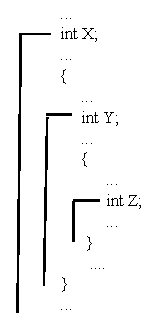
\includegraphics[width=9cm,height=6cm]{images/scope1.eps}}
\setlength{\unitlength}{1cm}
\begin{picture}(12,5)
\codefont{
\put(0.2,4.5){int main()\{}
\put(0.5,4.0){int x = 7;}
\put(0.5,3.5){int y;}
\put(0.5,3.0){\emph{y = foo(x);}}
\put(0.5,2.5){...}
\put(0.2,1.0){\}}
}

\put(4.2,4.3){The \emph{value} of \codefont{x} is copied into \codefont{z}}
\put(4.2,3.8){when the function is called.}
\linethickness{0.3mm}
\ifcolor\color{\mycolor}{
\put(4.1,3.6){\vector(1,0){5.5}}
\put(3.5,3.3){\line(1,0){0.5}}
\put(3.5,3.8){\line(1,0){0.5}}
\put(3.5,3.3){\line(0,1){0.5}}
\put(4.0,3.3){\line(0,1){0.5}}


\put(3.5,2.3){\line(1,0){0.5}}
\put(3.5,2.8){\line(1,0){0.5}}
\put(3.5,2.3){\line(0,1){0.5}}
\put(4.0,2.3){\line(0,1){0.5}}

\put(10,3.3){\line(1,0){0.5}}
\put(10,3.8){\line(1,0){0.5}}
\put(10,3.3){\line(0,1){0.5}}
\put(10.5,3.3){\line(0,1){0.5}}

\put(10,2.3){\line(1,0){0.5}}
\put(10,2.8){\line(1,0){0.5}}
\put(10,2.3){\line(0,1){0.5}}
\put(10.5,2.3){\line(0,1){0.5}}


\put(9.8,2.7){\vector(-1,0){5.5}}
\ifcolor}
\color{Black}{
\put(9.9,2.4){12}
\put(10.1,3.4){7}
\put(9.9,3.9){\codefont{z}}
\put(9.9,2.9){\codefont{a}}
\put(3.6,3.4){7}
\put(3.4,3.9){\codefont{x}}
\put(3.4,2.4){12}
\put(3.4,2.9){\codefont{y}}\put(0,0){\large\textbf{main() and its variables}}

%\put(7,0){\line(0,1){5}}

% ----------------  func
\codefont{
\put(11.5,4.5){\emph{int foo(int z)}\{}
\put(11.8,4.0){int a;}
\put(11.8,3.5){a = z + 5;}
\put(11.8,3.0){...}
\put(11.8,1.5){return a;}
\put(11.5,1.0){\}}
}


\put(4.4,2.3){The \emph{value} of \codefont{a} is copied into \codefont{y}}
\put(4.4,1.8){when the function returns.}

\put(10.5,0){\large{\textbf{foo() and its variables}}}
}
\end{picture}
\caption{When a function is called, the value of the arguments are copied into the function's parameters.  When a function returns, the return value (if any) should be copied into a variable in the calling function.}
\label{fig:arguments}
\end{figure}

Functions are defined as shown in Figure~\ref{fig:functions1}.
The return type of a function is the type (e.g., \codefont{int}) of value that the function returns.  If the function doesn't return a value, then the type is \emph{void}\index{void@{\cf{void}}}.  The function name is the name of the function.  Data may be passed to a function as arguments and stored in the function's parameters.  An ``answer'' can be returned via the return command.  A return statement can return a value (e.g., \codefont{return 7}) or a variable (e.g., \codefont{return X}), so long as the type of the returned value matches the return type in the function definition.  For example, on lines 8 and 9b, the return type of the function \codefont{get\_value()} is \codefont{double} (a new type) and the returned variable \codefont{temp\_value} has type \emph{\cf{double}} (declared on line 10b) and returned on line 13b.

The calculator program has four functions: \codefont{main()}\footnote{We have already seen that as a function, \codefont{main()} can return a value.  It turns out that \codefont{main()} can also receive arguments.  This is discussed in Interlude 6.}, \codefont{print\_menu()}, \codefont{get\_value()}, and \codefont{divide()}.  The \codefont{main()} function was already examined in Chapter 1.  The other functions are described in the following sections.

Functions must be called with the correct number and types of arguments.  When a program is compiled, the compiler checks whether functions are called with the correct number of arguments, which is only possible if it knows what the arguments should be; that is, it knows the functions' parameters.  This is the role of the \emph{prototypes}\index{prototype}.  Each of the three defined functions (\codefont{print\_menu()}, \codefont{get\_value()}, and \codefont{divide()}), has a prototype (on lines 7, 8, and 9, respectively).  A prototype defines the format of a function so the compiler can check that the function is being called properly.  For example, the prototype on line 9 tells the compiler that \codefont{divide()} must be called with two values or variables of type \cf{double} and should return a value of type \cf{double}.  If the \codefont{divide()} function is called with the wrong number or type of arguments, the compiler reports an error.  Another term for prototype is function \emph{declaration} because they are similar to a variable's declaration.  

\mysubsubsection{Pass-by-Value}\index{pass-by-value}\index{functions!pass-by-value}\index{arguments!pass-by-value}

An important aspect of parameters in C++ is that by default, they are \emph{pass-by-value}.  This means that the value of the argument is copied into the parameter in the function -- the function has access to the value, but \emph{not} the original ``box'' that the variable was stored in (see Figure~\ref{fig:arguments}).  Thus, any changes made to the value in the function are lost when the function exits, unless the new value is explicitly returned as part of the return statement.

For example, in the Calculator program on line 12b of the \codefont{get\_value()} function, the user's input is stored in the variable \codefont{temp\_value}.  However, to get that value back to the \codefont{main()}, the value must be returned (line 13b)  and stored in a new variable; for example, on line 23 where the returned value is stored in \codefont{operand1}.

An alternative approach to pass-by-value parameters is to use pass-by-reference parameters, which are discussed in Chapters 5 and 6.

\begin{figure}
%\centerline{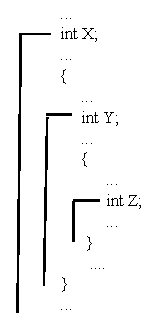
\includegraphics[width=9cm,height=6cm]{images/scope1.eps}}
\setlength{\unitlength}{1cm}
\begin{picture}(10,4)

\linethickness{0.3mm}
\put(2,2.5){\codefont{double divide(double dividend, double divisor)\{}}
\put(2.5,2){\codefont{code ...}}
\put(2.5,1.5){\codefont{return answer;}}
\put(2,1){\codefont{\}}}

\put(0.5,3.5){return type}
\color{\mycolor}{
\put(1.7,3.4){\vector(1,-1){0.5}}
\put(3.0,3.9){\vector(1,-2){0.55}}
\put(5.8,3.4){\vector(-1,-1){0.5}}
\put(7.9,3.4){\vector(1,-1){0.5}}
\put(7.4,2){\vector(-1,1){0.4}}
\put(8.9,2){\vector(2,1){0.8}}
\put(12.2,3.1){\vector(-2,-1){0.6}}
\put(2.85,0.7){\vector(-2,1){0.6}}
\put(5.95,1.2){\vector(-2,1){0.6}}
}

\color{black}{
\put(2,4){function name}
\put(5,3.5){parameter types}
\put(7.1,1.7){parameters}
\put(6.0,1.1){return statement}
\put(9.0,3.3){beginning \} starts the function}
\put(3,0.5){closing \} ends the function}
}

\end{picture}
\caption{The parts of a function definition. A function can have zero or more parameters, which may have different types.  A function has a return type (or \emph{void} if the function doesn't return a value).  A function may have several return statements in its code, but the first one reached returns a value and ends the function.}
\label{fig:functions1}
\end{figure}

\subsection{Functions with the Same Name}

In C++, it is legal to have two, or more, functions with the same name \emph{if they have different numbers or types of parameters}.  For example, two different divide functions could be defined with the following prototypes:\\
\codefont{
double divide(double dividend, double divisor);\\
double divide(double dividend, double divisor, double x);\\
}
The different type or number of parameters is necessary so that the compiler knows which function to call; that is, the function whose parameters match the arguments.  So, in the previous example, the command \codefont{divide(6.0, 2.5)} would be matched to the first version of the function and the command \codefont{divide(6.0, 2.5, 1.8)} would be matched to the second version of the function.


\subsection{Real Number Types}\index{double@{\cf{double}}}\index{type!double@{\cf{double}}}

The \codefont{double} type is used to store real numbers.  The term \cf{double} is derived from \emph{double precision}, which stands for a number that uses twice as much memory as a ``standard'' variable, which allows it to store more decimal places -- that is, to be more precise\index{double@{\cf{double}}}\index{type!double@{\cf{double}}}.  With the increase in the amount of memory that is cheaply available, \cf{double} has become the most common type for storing decimals in C++. Variables of type \cf{double} are stored in memory using scientific notation, with a fixed amount of memory reserved for the mantissa (or precision number) and a fixed amount of memory reserved for the exponent.  Because scientific notation is used, a double can represent a very large or very small number, but the precision is somewhat limited compared to the absolute size of the number (see Section~\ref{appendix:types} of Appendix A).  

\subsection{Conversions and Casts}\index{cast}\index{conversion}\index{promotion}

It is often necessary to convert the type of a value; for example, changing an \codefont{integer} into a \codefont{double} or vice versa.  This is most common in mathematical expressions that involve variables of more than one type.   For example, the code:\\
\cf{
int x = 11;\\
double var = 4;\\
var = x/var;\\
}
division is performed with an \cf{integer} (\cf{x}) and a \cf{double} (\cf{var}) and the result is stored in a \cf{double}.  What should the variable \cf{var} store?

C++ has implicit rules for converting between types (also known as casting).  There are two rules that are particularly important.  First, when operating on two different types C++ \emph{promotes} the lower precision value to the higher precision value.  So, in the previous example when \cf{x} is divided by \cf{var}, the value held by \cf{x} (e.g., 11) is temporarily promoted to a double (think of it as 11.0).  Thus, the division is treated as \cf{11.0/4.0} and the answer is 2.75, which is stored in \cf{var}.

Second, if a decimal value has to be stored in an integer type the value is \emph{truncated} (not rounded).  For example, if the previous code were changed to:\\
\cf{
int x = 11;\\
double var = 4;\\
x = x/var; // now the answer is stored in x\\
}
the division is the same (\cf{11.0/4.0 = 2.75}), but the answer has to be ``squished'' in to an integer (\cf{x}).  In this case C++ truncates the answer and \cf{x} ends up storing the value 2 (\emph{not} 3).

In understanding how C++ applies the first rule (when operating on two different types \emph{promote} the lower precision type to the higher precision type) it is important to realize that it is applied for each operation \emph{independently}.  For example, in the code:\\
\cf{
int x = 11;\\
double var = 4.5;\\
var = (x/12) * (x + var + 1000); \\
}
the variable \cf{var} will store the answer \emph{zero}.  The first operation C++ performs is \cf{x/12}, both \cf{x} and 12 are integers, so neither is promoted and the answer for that part of the calculation is truncated to zero, which leads to the final answer of zero.  A completely different answer is obtained simply by changing the calculation to:\\
\cf{var = (x/12.0) * (x + var + 1000); }\\
now the division (\cf{x/12.0}) is performed on an \cf{integer} (\cf{x}) and a \cf{double} (\cf{12.0}), the \cf{integer} is promoted to a \cf{double}, and that part of the expression is not truncated.  An alternative solution is to write the code as:\\
\cf{var = (double(x)/12) * (x + var + 1000); }\\
this tells C++ to treat the value in \cf{x} as a \cf{double} just for that part of the calculation.  (The variable \cf{x} is explicitly \emph{cast} as a \cf{double}.) In this case the 12 is also promoted to a double and the answer is not truncated.\footnote{Other languages treat mixed expressions with mixed types very differently.  For example, many languages \emph{require} explicit casting whenever two different types are combined. and will produce a compiler error otherwise.}

In creating expressions with mixed types it is very important to pay careful attention to how casting will work.  C++'s built-in rules for implicitly converting types, are only a guess at what the programmer intended and often give unexpected and undesired results.  Careful use of decimals and explicit casts will avoid a lot of program errors.  In addition, on many C++ compilers it is possible to increase the \emph{strictness}, which will cause the compiler to produce a warning whenever it identifies a piece of code that requires converting from a higher precision type to a lower precision type.  This can also be useful in avoiding difficult to identify errors causes by unexpected truncation in mathematical expressions with mixed types.


%-----------------------------------------------

\section{Analysis of the Code}

The general structure of the calculator program is relatively straight forward.  It consists of a main loop, similar to NIM, which allows the user to perform different calculations without having to restart the program.  Within this loop is a menu structure that allows the user to select which operation to perform.  A switch statement is used to process the user's choice.  Additional functions, like \codefont{get\_value()}, simplify the code for each of the user choices.
%General description of the code

\mysubsubsection{Lines 1-3: Comment Block}
As with the NIM program, these lines are a comment block briefly describing what the program does.

\mysubsubsection{Lines 4-5: \#includes}
As with the NIM program, these lines are preprocessor commands that include necessary libraries.

\mysubsubsection{Lines 7-9: Function Prototypes}

These are the prototypes for the functions \codefont{print\_menu()}, \codefont{get\_value()}, and \codefont{divide()}.  The prototypes declare a function's name, parameters, and return type. 

An alternative approach is to write the entire function definition before the \codefont{main()} function.  In this case, the prototype is not required because the compiler has access to the entire function definition right from the start.  There are two problems with this approach.  First, it's not considered good programming practice.  Second, if the code has two functions that call each other (e.g., function \codefont{A()} calls function \codefont{B()} and function \codefont{B()} calls function \codefont{A()}) then it is necessary to have prototypes.  Otherwise, the compiler will give an error in whichever function comes first in the code, because the compiler will not have seen the other function's definition.

A third approach, discussed in Chapter 7, is to place the function code in a separate, user-defined library.  This is useful when the functions are general-purpose and may be used in many different programs. 

\mysubsubsection{Lines 1b-22b: Function Definitions}

The code for the functions is presented in Listing~\ref{listing:calcFunctions}.

The \codefont{print\_menu()} function (lines 16b-22b) is the simplest of the functions.  It doesn't take any arguments; that is, no data is passed to the function, and it doesn't return a value.  So, on line 16b, where \codefont{print\_menu()} begins, the return type is \emph{void} and there is nothing inside the parentheses.  The function consists of a series of output commands.  When the function is called, it generates some output and, when it reaches the function's last \} on line 22b, it returns to the place in the code where it was originally called from.  The output commands could have been put in the main function, but by making a separate function, the program is divided into more readable blocks.

The next simplest function is \codefont{get\_value()}, defined on lines 9b-14b.  It also doesn't take any arguments, but it does return a value (of type \codefont{double}).  Thus, on both lines 8 and 9b, the return type for the \codefont{get\_value()} function is \codefont{double}.  The function itself creates a variable called \codefont{temp\_value} (line 10b), gets a value from the user that is stored in \codefont{temp\_value} (line  12b), and then returns that value (line 13b).  

Thus, when the program gets to line 23 (or line 24, 28, or 29), it jumps to the \codefont{get\_value()} function that starts on line 9b.  The \codefont{get\_value()} function gets a value from the user (line 12b) and then returns it (line 13b).  Back on line 23, the returned value is stored in the variable \codefont{operand1} (or \codefont{operand2} on lines 24 and 29).  Notice that the names of the variables are different because two different ``boxes'' are involved: a box/variable called \codefont{temp\_value} in the function and a box/variable called \codefont{operand1} (or \codefont{operand2}) in main; only the \emph{value} that was stored in \codefont{temp\_value} is copied from the function to the variable in main.  

Note that in the \cf{main()} function, the \codefont{get\_value()} function is called in several places (lines 23, 24, 28, and 29).  This is one of the major advantages of a function -- instead of having to write the same piece of code over and over, it can be written once as a function and then called whenever it is needed.

\begin{wrapfigure}{R}{0.5\textwidth} \framebox[\linewidth][l]{\parbox{0.9\linewidth}{\codefont{Matching Arguments and Function Calls} \\
When a function is called, it is critical that it is passed the correct number and type of variables.  For example, whenever the divide function is called, it \emph{must} receive two values of type \cf{double}.  Thus, on line 30, where \codefont{divide()} is called, there must be two values or variables of type \cf{double} in the parentheses to match the two arguments on line 2b.  Mismatched arguments are a common error in programming.  
}}
\vspace{-0.5cm}
\end{wrapfigure}

The \codefont{divide()} function, lines 2b-7b, has both a return value and two parameters, all of which have the type \codefont{double}.  The two parameters are named \codefont{dividend} and \codefont{divisor}.  These variable names are not the same as are used when calling the function from \codefont{main()} (line 30).  The variables in the calling function (in this case, \codefont{main()}) and in the called function (in this case, \codefont{divide()}) are independent -- only the values are copied from the calling function to the called function. 

After receiving its arguments, the \codefont{divide()} function begins by checking whether the divisor is zero (line 3b).  If a C++ program tries to divide by zero, the results are unpredictable and the entire program may crash\index{divide by zero}.  Thus, it is important to make sure that the divisor is not zero before doing the division on line 6b.  If the divisor is \emph{not} zero, the program divides and returns the answer in one step.  However, if the divisor is zero, the program still has to return a value (that's the way the function is defined, it returns a \cf{double}), so as a temporary solution, it returns a zero (line 4b).

The \codefont{divide()} function has two return commands on lines 4b and 6b.  As soon as one of them is reached, the program \emph{returns} to where it was called from and none of the code after the return command gets executed.  

\mysubsubsection{Lines 11-12, 41: Main}

Lines 11-12, and 41 define the \codefont{main()} function.  The syntax of the \codefont{main()} function should now be a little clearer.  It takes no arguments (although this can be changed -- see Interlude 6), and it ends by returning a 0 on line 40.

\mysubsubsection{Lines 13-14: Variables}

Lines 13-14 declare the variables used in the \codefont{main()} function.  Note that, three variables (\codefont{operand1}, \codefont{operand2}, and \codefont{answer}) are declared simultaneously on line 13.  So long as the variables have the same type, they can be declared together.  

\mysubsubsection{Lines 15-39: The Calculator Loop}

Lines 15 and 39 define a \cf{do-while} loop similar to the one used in NIM in Chapter~\ref{ch:NIM}.  This loop allows the program to perform repeated computations until the user is done.  The termination condition for the loop, part of the \cf{while} command on line 39, is:\\
\codefont{choice != 0}\\
This is true so long as the value stored in the variable \codefont{choice} is \emph{not} equal to 0 (the character pair != stands for not equal).  Therefore, so long as the user's choice is not zero, the program will continue to loop, and when the user chooses 0, the loop ends.

\mysubsubsection{Line 16: Print Menu}

Line 16 calls the \codefont{print\_menu()} function.  The computer jumps to the beginning of that function and begins running the code within the function, which prints the menu options to the screen.  The function ends when when it reaches the closing \} on line 22b and the computer jumps back to line 16 where the function was called.

\mysubsubsection{Line 18: A Valid Choice}

Line 18 sets the value of the variable \codefont{valid\_choice} to 1.  As the comment (everything after the //) explains, a 1 means that the computer ``thinks'' the user has entered a valid menu option.  If this is not true, the value is changed to 0 later in the code.  On line 36, the value stored in \codefont{valid\_choice} is used to determine whether the answer should be printed.  If \codefont{valid\_choice} is 1, meaning the user made a valid choice from the menu options, the answer is printed.  If the value of \codefont{valid\_choice} is 0, meaning the user did not make a valid choice, the answer isn't printed.

\mysubsubsection{Lines 19-35: Switch Statement}\index{switch@{\cf{switch}}}

Line 19 is the beginning of a switch statement.  A \emph{switch} statement is a conditional statement like an if-else statement.  It is particularly useful when there are multiple, discrete options, as in a menu.   
%A switch statement takes an integer type as input and then jumps to the matching \emph{case}\index{case}.

The general format of a switch statement is:\\
\codefont{
switch(\emph{variable})\{\\
\hspace*{0.5cm}      case 1:\\
\hspace*{1.0cm}  \emph{code block 1}\\
\hspace*{1.0cm} break;\\
\hspace*{0.5cm}   case 2:\\
\hspace*{1.0cm}  \emph{code block 2}\\
\hspace*{1.0cm}   break;\\
\hspace*{0.5cm}    ...\\
\hspace*{0.5cm}    default:\\
\hspace*{1.0cm}  \emph{code block N}\\
\hspace*{1.0cm}   break;\\
\}\\
}
When the \codefont{switch} is reached, the value of \codefont{\emph{variable}} is checked and the program jumps to the matching \emph{case}\index{case@{\cf{case}}}.  For example, if the variable's value is 3, then the program jumps to case 3.  If there is no matching case, then the program jumps to the \emph{default}\index{default@{\cf{default}}} case.  Typically, the cases are positive and in order (1, 2 , 3, etc.) but any integer values in any order will work.\footnote{Switch statements can also use a variable of type \codefont{char}, which is short for \emph{character} and will be introduced in Chapter 5.} 

Each case ends with a \codefont{break}\index{break@{\cf{break}}} statement.  When the program reaches a break statement, it jumps to the end of the switch statement: the closing \}.  Without the break statement, the program will ``fall through'' the other cases and execute them as well.\footnote{Break statements can also be used to break out of loops or conditionals.  However, this is generally considered to be poor programming practice and should be avoided.}  For example, without breaks, if the variable had the value 2, the program would jump to case 2, but then it would continue to execute case 3, case 4, etc., all the way through the default case.  

The case statement can only have a single, fixed value.  Statements like:\\ \codefont{case <5:} and \codefont{case 4 to 10:} \\will \emph{not} work.  One approach that does work is to ``stack'' cases:\\
\codefont{
case 2:\\
case 3:\\
case 4:\\
\hspace*{0.5cm} \emph{code ...}\\
\hspace*{0.5cm} break;\\
}
This will result in the same code being applied to cases 2 through 4.

\mysubsubsection{Lines 20-21: Case 0}
If the user enters a 0 (for exit), the switch statement just executes a break and jumps to the end of the switch statement.  From there, the \cf{do-while} loop ends, because the variable \codefont{choice} has the value 0, which causes the main loop to end.  %Alternatively, the program could end immediately by putting \codefont{return 0;} on line 21.

\mysubsubsection{Lines 22-26: Case 1}
If the user enters a 1 (for addition), the program uses the \codefont{get\_value()} function twice to get two numbers from the user and stores them in the variables \codefont{operand1} and \codefont{operand2}.  Then it adds them and stores the result in the variable \codefont{answer} (line 25) to be printed later (line 37).  Finally, the break statement causes the program to jump to the end of the switch statement (line 35).

\mysubsubsection{Lines 27-31: Case 2}
If the user enters a 2 (for division), the program uses the \codefont{get\_value()} function twice to get two numbers from the user and stores them in the variables \codefont{operand1} and \codefont{operand2}.  Then it divides them using the divide function and stores  the result in the variable \codefont{answer} (line 30) to be printed later (line 37).  Finally, the break statement causes the program to jump to the end of the switch statement (line 35).

\mysubsubsection{Lines 32-34: Default}

If the user enters any value besides 0, 1, or 2, the program jumps to the \emph{default} case.  There, the variable \codefont{valid\_choice} is set to 0, for false, and the message \codefont{Invalid Choice} is printed to let the user know that he or she entered an invalid choice.  The variable \codefont{valid\_choice} is set to 0, which keeps the program from printing an answer when it reaches line 36. 

Including a default case is not required in C++, but it is a very good idea.  Even if you are sure that every possible case is covered without the default, including a default case that prints an error message makes debugging the code much easier if an unexpected case does occur.

\mysubsubsection{Lines 36-38: Print the Answer}

Line 36 uses an if statement to check whether the user entered a valid menu choice.  A common C++ trick is used in the condition in line 36.  Instead of comparing \codefont{valid\_choice} to 0 or to 1 the conditional in the if statement  is just the variable \codefont{valid\_choice}.  In C++, any zero value is considered false, and any nonzero value is considered true.  So, on line 36, if \codefont{valid\_choice} is 1, it is considered \emph{true} and the answer is printed.  If \codefont{valid\_choice} is 0, from line 33, then it is considered \emph{false} and the \codefont{cout} statement is skipped.

\subsection{Scope}\index{scope}

\begin{wrapfigure}{R}{0.5\textwidth} \framebox[\linewidth][l]{\parbox{0.9\linewidth}{\codefont{Scope, Variable Names, and Team Projects} \\
Most commercial software products are written in separate blocks by members of a large team.  Scope separates variables in different blocks of code.  For example, the variable \codefont{X} in one block of code is independent of any other variables called \codefont{X} declared in other blocks of code.  Thus, in a large programming project any programmer is free to select their own variable names without having to worry about them conflicting with variables in another part of the program -- as long as the scope of the variables don't overlap.
}}
\vspace{-0.5cm}
\end{wrapfigure}

In this program, there are variables in \codefont{main()} and variables in most of the functions.  Some of these variables may have the same name, but they don't represent the same ``box.''  If they did represent the same ``box'' it would become very confusing, especially in  large programs written by teams of programmers.  No one would ever know which variables had already been created elsewhere in the code or where else in the code the values for ``their'' variables might be changed.

\emph{Scope} solves this problem by limiting the regions of code in which a particular variable is valid and can be used.  The basic rule for the scope of a variable is simple: a variable's scope extends from where the variable is declared to the right curly brace \} ending the block of code that the variable is declared in (see Figure~\ref{fig:scope1}).

\begin{figure}
%\centerline{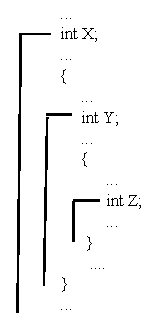
\includegraphics[width=9cm,height=6cm]{images/scope1.eps}}
\setlength{\unitlength}{1cm}
\begin{picture}(8,7)
%\codefont{
%\linethickness{0.3mm}

\put(1.5,6.5){int main()\{}
\put(2,6){\emph{int \codefont{X};}}


\put(2,5.5){\{}
\put(2.5,5){code ...}
\put(2.5,4.5){\emph{int \codefont{Y};}}
\put(2.5,4){code ...}
\put(2.5,3.5){\{}
\put(3,3){code ...}
\put(3,2.5){\emph{int \codefont{Z};}}

\put(3,2){code ...}
\put(2.5,1.5){\}}
\put(2.5,1){code ...}
\put(2,0.5){\}}

\put(1.5,0){\}}

% ---- func

\put(6.5,6.5){int func(int X)\{}
\put(7,6){\emph{int \codefont{Y};}}
\put(7,5.5){code ...}
\put(6.5,3){\}}

\ifcolor\color{\mycolor}{
\put(0.88,5.1){\codefont{X}}
\put(1.5,3.9){\codefont{Y}}
\put(2.05,2.1){\codefont{Z}}
\put(6.05,5.9){\codefont{X}}
\put(6.55,5.2){\codefont{Y}}

\put(1.3,6.2){\vector(0,-1){5.7}}
\put(1.8,4.7){\vector(0,-1){3.7}}
\put(2.3,2.7){\vector(0,-1){1.2}}

\put(6.3,6.6){\vector(0,-1){3.2}}
\put(6.8,6.2){\vector(0,-1){2.8}}
\ifcolor}

\end{picture}
\caption{Illustration of scope.  The vertical lines mark the scope of each of the variables \codefont{X}, \codefont{Y}, and \codefont{Z} (including second variables \cf{X} and \cf{Y} in the function).  Scope extends from the where the variable was declared to the closing bracket \} marking the end of that block of code.  Note that scope includes any nested blocks, for example, \codefont{Y}'s scope includes the nested set of brackets \{\} where \codefont{Z} is declared, and \codefont{X}'s scope includes the scope of both \codefont{Y} and \codefont{Z}.   Any reference to a variable outside of its scope will result in a compiler error or warning.  The variables \codefont{X} and \codefont{Y} in the function \codefont{func()} have their own scope and are separate from the variables of the same name in \codefont{main()}. }
\label{fig:scope1}
\end{figure}

Any reference to a variable outside that variable's scope is an error that will be caught and reported by the compiler.  One way to think of this is that when a program reaches the end of a variable's scope, the ``box'' corresponding to that variable is destroyed.\footnote{Actually, when a variable reaches the end of its scope, the variable is no longer usable, but the value it stored is often left in memory, where it's hard, but not impossible, to access.  This can lead to security problems if the value needs to be secure.  Thus, in sensitive programs, it's a good idea to ``zero out'' a variable's value before leaving its scope.}  Another variable of the same name could be declared somewhere else in the code, but this would be a separate box, with no connections to the original variable of the same name.

Scope is particularly important in using functions.  The scope of a variable only extends to the function it was declared in.  For example, in the calculator program, there is a variable called \codefont{answer} declared in \codefont{main()} on line 13.  This variable cannot be used in any of the functions.  The value of \codefont{answer} cannot be set, and its value cannot be accessed, from any of the functions.  

To test the scope of the variable \codefont{answer}, try the following.  Replace line 6b of the program with the following new line:\\
\codefont{answer = dividend/divisor;}\\
This may appear to set \codefont{answer} to the correct value so it can be printed in \codefont{main()}.  Instead a compiler error is generated because the scope of  \codefont{answer} does not extend to the function \codefont{divide()}.  That's why the function \codefont{divide()} has to return the correct value, so that it can be stored in the variable \codefont{answer} on line 30.

Whenever a function is created it's important to think about what data is being sent to the function (the arguments) and what data, if any, the function is returning.  Carefully planning the data flow for a function before beginning to program it will avoid many potential errors.

% box globals
\vspace{+0.25cm}
{\color{\mycolor}\noindent\hrulefill}
\section{Exercises: Modifying the Program}
By now, you should have a general idea of how the program works.  However, there are many changes and improvements that can be made.  The suggested modifications begin with a few simple changes before moving on to more complex and more interesting changes.  Not all of the new code will be given, in many places, only suggestions about how to proceed are provided.

\mysubsubsection{Exercise 1: Modifying the Output}

Add some initial output printing information about the program: the name of the author (you), the date it was created, and a brief explanation of its functionality.  This is done with one or more \codefont{cout} statements that print the desired information near the beginning of the program.  

\mysubsubsection{Exercise 2: The Final Answer}
Fix the minor, but annoying, problem that when the user exits, the program reprints the last answer.  
The best way to fix this flaw is to use the existing conditional on line 36.  One option is to expand the condition so that it prints the answer only if the user made a valid choice and didn't choose to exit, making the condition\\
\codefont{valid\_choice \&\& (choice != 0)}\\
Alternatively, case 0 could be modified to make \codefont{valid\_choice} 0, which would also keep the answer from being printed.  Note that both of these solutions have the advantage of using the conditional that's already part of the program rather than having to add a lot of new code.

\mysubsubsection{Exercise 3: Printing Answers and Problems}
Currently, the program just prints the answer to each of the user's problems.  Change the output so that the program prints the whole problem as a mathematical expression.  For example, if the user asks for the sum of $4.5$ and $1.3$, the program currently prints:\\
\codefont{answer = 5.8}\\
whereas it could print:\\
\codefont{4.5 + 1.3 = 5.8}\\
Changing line 37 to something like:\\
\codefont{cout << operand1 << "???" << operand2 << " = " << answer << endl;}\\
works except for the ??? part.  What should go there?  The problem is that the program has ``forgotten'' which operation the user picked.  One approach is to replace line 37 with another switch statement based on the \codefont{choice} variable, such as\\
\codefont{
switch(choice)\{\\
\hspace*{0.5cm}case 1: \\
 \hspace*{1.0cm}         cout $<<$ operand1 $<<$ "+" $<<$ operand2 $<<$ " = " $<<$ answer $<<$ endl;\\
   \hspace*{1.0cm}       break;\\
\hspace*{0.5cm}     case 2:\\
  \hspace*{1.0cm}           cout $<<$ operand1 $<<$ "/" << operand2 $<<$ " = " $<<$ answer $<<$ endl;\\
 \hspace*{1.0cm}            break;\\
...\\
\}\\
}
Then for each choice, the program prints the correct output (the default case wouldn't print anything because it's an invalid choice).

However, the code already contains a switch statement very similar to this one.  Reusing the existing switch statement will shorten the program and adding more options will only require changing one switch statement, not two.  To use the existing switch statement, the first part of the output is printed within the switch statement and the answer is still printed on line 37.  For example, an extra line would be added between lines 25 and 26:\\
\codefont{cout << operand1 << "+" << operand2 << " = ";}\\
and a similar line would be added between lines 30 and 31:\\
\codefont{cout << operand1 << "/" << operand2 << " = ";}\\
Note that these have the correct operator, but they don't print the answer yet (although they could).  Then line 37 would be changed to just\\
\codefont{
cout << answer << endl;}\\
This way, the mathematical expression is printed from one line and the answer is printed from a very different line, but because of the way the spacing is used, it looks like one expression in the output.
         
\mysubsubsection{Exercise 4: More Functionality -- Subtraction}

Of course, the biggest drawback to this calculator is that it can only do two things: addition and division.  However, the program was designed to make it (fairly) easy to add other functions.  Add an option that allows the user to perform subtraction.  

This requires two changes.
First, subtraction needs to be added as an option in the \codefont{print\_menu()} function.  This just requires adding a line like\\
\codefont{cout << "Subtract (3)" << endl;}\\
around line 19b.

Second, a new case (case 3) needs to be added to the switch statement that starts on line 19.  Copy the addition case (lines 22-26), change the case number from 1 to 3, and the operation from addition to subtraction.  It is a good idea to rearrange and renumber the menu options so that the operations are in a more natural order, making sure that the choices in the menu match up with the cases in the switch statement.

\mysubsubsection{Exercise 5: More Functionality -- Minimum}

\begin{wrapfigure}{R}{0.5\textwidth} \framebox[\linewidth][l]{\parbox{0.95\linewidth}{\codefont{The cmath Library}\index{libraries!cmath@{\cf{cmath}}}\index{cmath@{\cf{cmath}}} \\
In addition to the mathematical operators already described and listed in Section~\ref{appendix:operators} of Appendix A there is a C++ library called \codefont{cmath} that defines many additional mathematical functions: sine, cosine, square root, etc.  These are actual functions; for example to calculate the sine of a variable called \codefont{angle}, the command would be:
\codefont{sin(angle);}  To include the library, add the line:
\codefont{\#include$<$cmath$>$}
with the other include statements.
Using the math library, the calculator program can be expanded to include many more functions.  The full details of the \codefont{cmath} library can be found online.
}}
\vspace{-0.0cm}
\end{wrapfigure}

Add a minimum operation that prints the minimum of two values entered by the user.  The minimum should be calculated by calling a function (like the current \codefont{divide()} function) that will need to be written as well.  (In general, a function should be used when more than a few lines of code are necessary to perform the calculation.)

The first steps are to add the new option in the \codefont{print\_menu()} function and to add a new case to the switch statement.  The new case should call a function called \codefont{minimum()}.  The new case should be similar to the divide case (lines 27-31), but the case number needs to be changed and instead of calling  \codefont{divide(operand1,operand2)}, the new case should call \codefont{minimum(operand1,operand2)}.  

Next, the \codefont{minimum()} function needs to be written.  Start by copying the divide function (lines 2b-7b).  Name the new function \codefont{minimum}.  The parameters (\codefont{dividend} and \codefont{divisor}) should be renamed to be more appropriate to the function.  The if-else statement (lines 3b-6b of the original function) need to be rewritten to return the minimum value.  The resulting function could look like\\
\codefont{
double minimum(double value1, double value2)\{\\
\hspace*{0.5cm} if(value1 < value2)\\
\hspace*{1cm} return value1;\\
 \hspace*{0.5cm} else\\
\hspace*{1.0cm} return value2;\\
\}\\
}
where, in this case, the new parameters are \codefont{value1} and \codefont{value2}, but they could be anything. 

Finally, a new prototype needs to be added so the compiler can check that the function is being used properly.  The prototype needs to be listed with the other prototypes somewhere between lines 7 and 9.  It should be:\\
\codefont{double minimum(double, double);}\\
Note that the prototype specifies the function name, number, and type of the parameters, as well as the return type.  

Now the \codefont{minimum()} function should be working. Run the program and choose the minimum option to test whether it works correctly.  Remember to check what happens if the user enters two values that are identical.  It's good practice to try to figure out what will happen by looking at the code before testing the results.

\mysubsubsection{Exercise 6: Absolute Value}

So far, all of the operators discussed (add, subtract, multiply, divide, and minimum) have had exactly two operands.  This is not a requirement.  A different operation might need one operand or three or more operands.  Note  that if a function requires more than two operands, additional variables (\codefont{operand3}, \codefont{operand4}, etc.) need to be declared on line 13.

Add an absolute value operation (an option that returns the absolute value of a number) to the calculator.  Because it calculates the absolute value of only one number, the \codefont{get\_value()} function only needs to be called once.  

\mysubsubsection{Exercise 7: Cartesian Distances}

Create an option that calculates the distance between two points in a Cartesian plane.  This option needs four values: the $x$ and $y$ value for each of the two points.  Once the four values are input by the user, write a new function that will accept the four values as arguments and calculate and return the distance between them.

%Functions calling other functions

\section{Problems}

The potential for extending the calculator program should now be clear.  Additionally, the basic framework, particularly the menu, can be used as the basis for many other programs.  The following problems explore these possibilities.

\begin{enumerate}[{\bf 1.}]
\item {\bf More complex operations} \\
Use the \codefont{rand()} function to create an option to generate random numbers, with one input from the user to determine the maximum random number.  (Review Chapter~\ref{ch:NIM} to see how to use the modulus operator to control the range of random numbers.)  

\item {\bf Customized calculator} \\
Customize the program for a particular application domain, such as geometry, chemistry, or physics.  Add at least three new calculations that are specifically designed for the new application.  For example, if the new calculator is designed for geometry applications add options for calculation areas, perimeters, etc.  Make sure the menu options are clear and that the program begins with some (brief) output explaining the calculator's purpose.
  
\item {\bf Reusing answers}\\
 Currently the calculator can perform only one calculation at a time.  Change the program to allow the user to use the previous answer directly as input for the next calculation without having to retype the answer.  For example, if the user adds two numbers, the sum can be used directly in the next calculation without reentering it.   Write the code so that after the program calculates an answer, it asks the user whether he or she wants to reuse that value and, if the user answers yes, \codefont{operand1} is set equal to the answer (instead of requesting a new \cf{operand1}) for use in the next calculation.  

\item {\bf Unlimited inputs}\\
 For some operations, it's not known in advance how many values the user wants to input.  For example, in an averaging operation, the user may want to average any number of values.  Create an \codefont{average()} function, like the \codefont{divide()} function, that has its own loop within the function for entering values.  The user should enter values one at a time, and after each value, the program asks whether the user wants to enter another value.  The program should keep a running sum of the values and the number of values entered to know what to divide by when the user stops entering values.

\item {\bf Menus in NIM}\\
Rewrite the NIM program so that users are given a menu of possible moves.  In the basic NIM game the options should be to remove one, two, or three objects.  The menu should not give illegal options, for example having the option to remove three objects when there are only two objects left.\\
{\bf Challenge:} Using the rules for making the computer play NIM intelligently (Exercise 6 of Chapter 3) have the program give the user hints as part of the menu options. 

\item {\bf Functions in NIM}\\
Rewrite the NIM program to use functions.  Create at least the two functions.  The first function should choose the computer's random move; the function should take the number of remaining objects as an argument and return a legal move.  The second function should allow the player to select their move; the function should take the number of remaining objects as an argument and only return a legal move.  

\item {\bf A Roulette game} - The basic calculator framework can be reused for other purposes.  Create a Roulette game in which the menu items correspond to potential bets: red, even, specific numbers, etc.  After the user has picked a bet, the program uses the \cf{rand()} to determine the outcome and reports whether the user won or lost.  \\
{\bf Challenge:} Allow the user to choose how much to bet and have the program keep track of the user's current bankroll (similar to the way the NIM game kept track of the objects remaining).

\item {\bf A sports strategy game} \\
Create a sports strategy game, where the menu helps the user pick a move (e.g., run or pass in a football game, or jab, hook, or block in a boxing game), then the computer picks a random countermove, and the outcome is based on the opposing moves.\\
{\bf Challenge:} Add a random factor to the outcomes.  For example, if the the user chooses to pass and the computer chooses to blitz (in a football game) it may be very likely that the user will lose a little yardage, but there's a small chance that they will gain a lot yardage.
\end{enumerate}